\newpage
\section{Degustation}
\subsection{Planung}
\subsubsection{Ziele der Degustation}
\begin{itemize}
    \item Erkennen die Befragten den Unterschied zwischen alkoholfreiem und alkoholhaltigem Bier?
    \item Können wir als Anfänger ein vergleichbares Bier herstellen?
    \item Wie wird unser Bier bewertet?
\end{itemize}
Das Auswertungsblatt ist in den Beilagen sichtbar.
\subsubsection{Durchführung}
Wir verwenden Plastikbecher und markieren diese mit folgendem Farbschema:
\begin{itemize}
    \item Blau: 	Selbstgebrautes Weizenbier
    \item Rot:		Selbstgebrautes Cherry Ale
    \item Gelb: 	Feldschlösschen Braufrisch \footcite[Internet shop - Braufrisch Bier 6 x 0.5 l]{brack}
    \item Grün:		Chouffe Cherry Ale \footcite[CHOUFFE Cherry]{Manor}
    \item Schwarz:	Appenzeller Weizenbier (Alkoholfrei) \footcite[Appenzeller Bier Sonnenwendlig alkoholfrei]{Coop}
\end{itemize}

Danach werden die Biersorten in die dafür vorgesehenen Plastikbecher abgefüllt. Es soll somit vermieden werden, dass die Teilnehmer wissen, um welches Bier es sich jeweils handelt.
Wir bitten die Teilnehmer dann jeweils eine Biersorte nach der anderen zu probieren und dabei das Auswertungsblatt, welches weiter unten zu finden ist, auszufüllen. Mit dieser Methode ist es uns möglich herauszufinden, ob die Testpersonen unser Bier mögen oder einen Unterschied von alkoholhaltigem und nicht alkoholhaltigem Bier herausschmecken können. Weiter werden wir bei der Wahl darauf achten, möglichst unterschiedliche Altersgruppen und Alkoholkonsumenten einzuladen, so dass wir gegebenenfalls einen Unterschied zwischen Altersgruppen und den verschieden starken Alkoholkonsumenten herausfinden können.
\\\newpage
\textbf{Design:}\\
Aktuell haben wir nur die «nackten» Bierflaschen. Da wir aber bei der Degustation und vor allem auch bei der Präsentation einen ästhetisch ansprechenden Auftritt liefern wollen, haben wir und dazu entschieden Labels für die Flaschen zu erstellen. Diese Aufgabe haben wir mit Photoshop und Etikettenpapier bewältigen. Wir haben mehrere Designs erstellt und uns für die zwei folgenden entschieden:

\begin{figure}[!h]
    \centering
    \begin{minipage}{.5\textwidth}
      \centering
      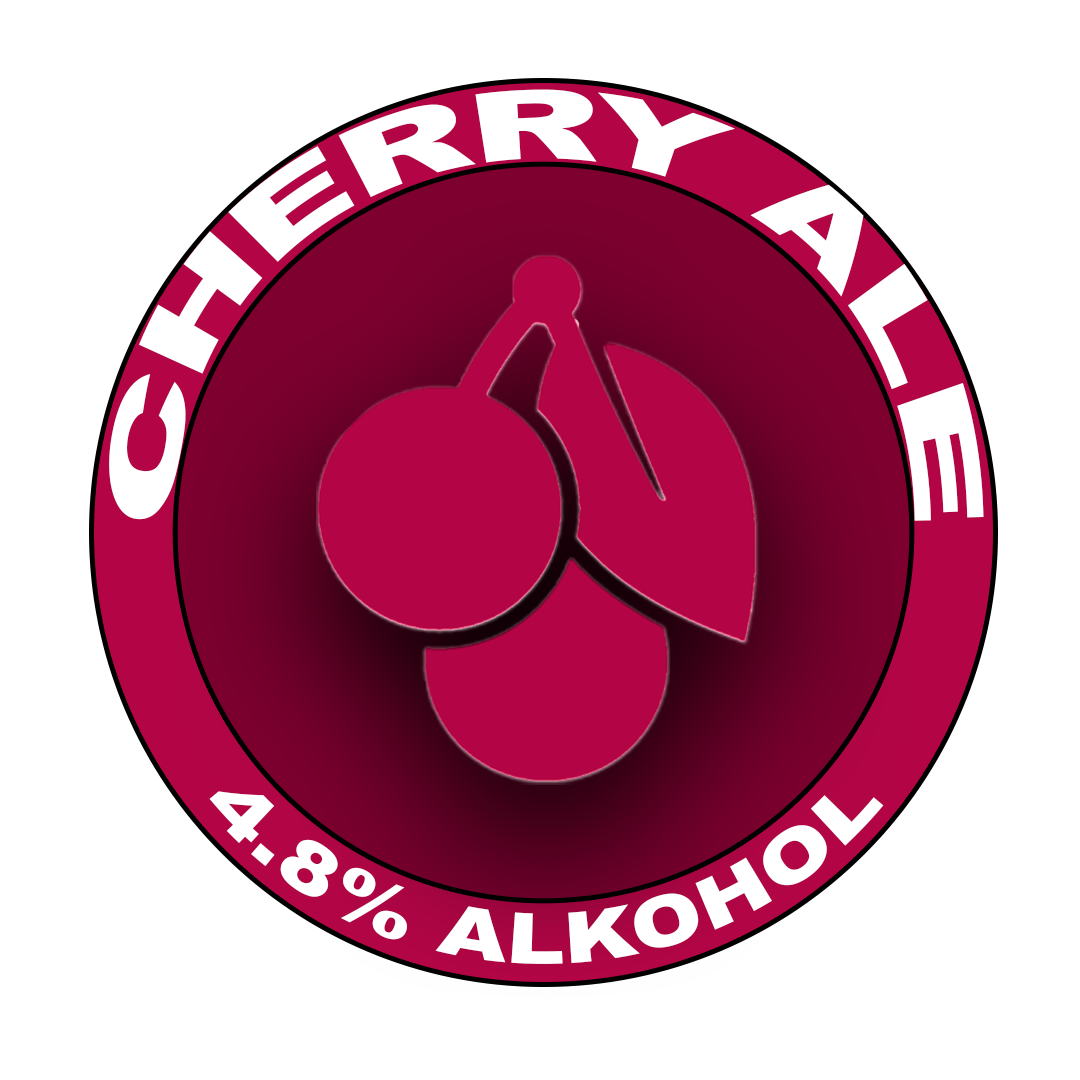
\includegraphics[width=.7\linewidth]{Cherry.png}
      \captionof{figure}{Cherry Ale Design}
      \label{fig:test1}
    \end{minipage}%
    \begin{minipage}{.5\textwidth}
      \centering
      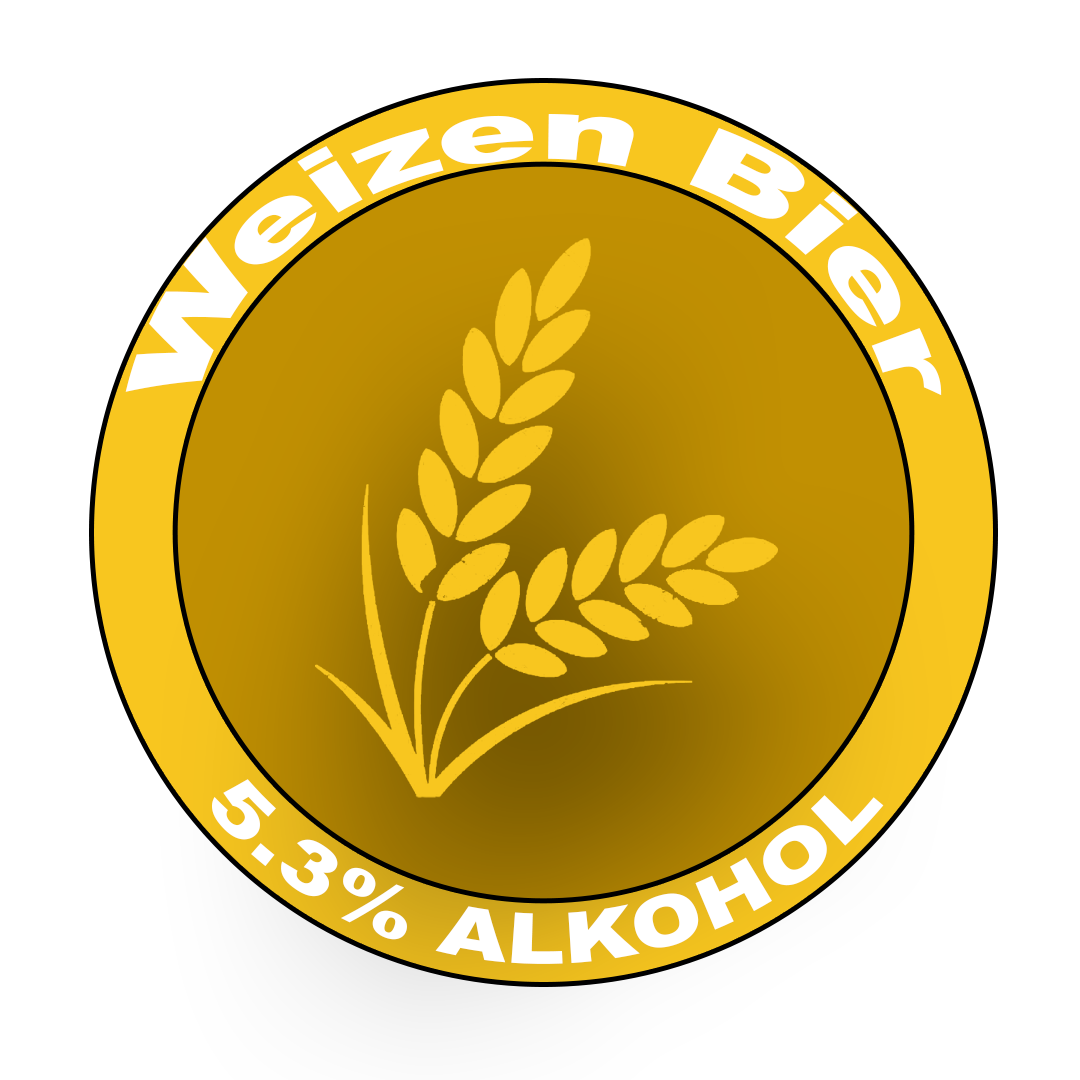
\includegraphics[width=.7\linewidth]{Figures/Wheat.png}
      \captionof{figure}{Wheat Design}
      \label{fig:test2}
    \end{minipage}
\end{figure}

\textbf{Allgemein:}\\
Es war uns wichtig, dass das Design simpel und ansprechend aussieht. Dazu waren wir limitiert, da unser Etikettenpapier uns nicht viel Platz bat. Da wir das Bier nicht kommerziell nutzen, mussten wir auch keine Angaben über die Inhaltsstoffe andrucken, was uns natürlich viel Ärger erspart hat. Der Äussere Ring dient als Platzhalter für den Titel und den Alkoholgehalt. In der Mitte haben wir einen dunkleren Hintergrund und das Logo, welches mit einem leichten Schlagschatten heraussticht.
\\
\textbf{Cherry Ale:}\\
Die Kirsche vom Cherry Ale Logo wurde von dem Unternehmen «MX CHERRY» \footcite[Die besten Schalter für mechanische Tastaturen]{Cherry}  inspiriert. Farblich haben wir uns für ein dunkles Weinrot entschieden, da wir fanden, dass das zu Kirschen passen würde. Der kapitalisierte und verzerrte Titel sorgt für Aufmerksamkeit und das Logo sticht von der Mitte hervor.
\\
\textbf{Weizen Bier:}\\
Beim Weizenbier wollten wir natürlich auch in dem gleichen Stil bleiben, jedoch sollte jedermann einen klaren Unterschied zwischen den Biersorten erkennen. Dies haben wir mehrheitlich durch die Farbe und dem Symbol erzeugt. Hier haben wir die Kapitalisierung des Titels weggelassen, um dem Symbol eine grössere Aufmerksamkeit zu widmen. 

\newpage
\subsection{Auswertung}
Aus den Daten der Auswertung konnten wir folgendes Herausfinden:
\begin{figure}[!h]
	\centering
	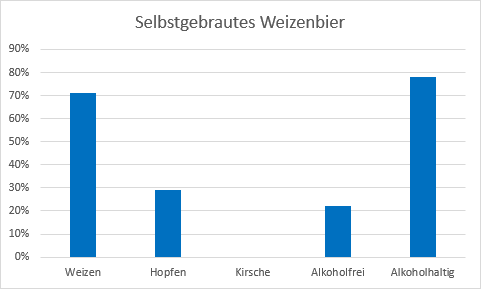
\includegraphics[width=0.5\columnwidth]{swt.png}
	\caption{Selbstgebrautes Weizenbier Tabelle}
\end{figure}
Das selbstgebraute Weizenbier wurde mehr als zwei Drittel als Weizenbier erkannt. Das liegt wahrscheinlich daran, dass das Weizenbier bei uns im Freunden- und Familienkreis das beliebteste Bier ist. Überraschender Weise konnten doch fast 30 Prozent der Befragten das Weizenbier nicht als solches erkennen,
 sondern als Hopfenbier. Daraus können wir erkennen, dass fast jeder dritte das Bier nicht unbedingt am Geschmack, sondern an dem Label erkennt. Weiter wurde unser Bier von 22 Prozent der Befragten als Alkoholfreies Bier bezeichnet. Durch Rückfragen mit den Befragten konnten wir herausfinden,
 dass dies daran liegt, dass das Bier Ihnen «fremd» geschmeckt hat und manchen einfach die Erfahrung eines alkoholfreien Biers gefehlt hat.
 \begin{figure}[!h]
	\centering
	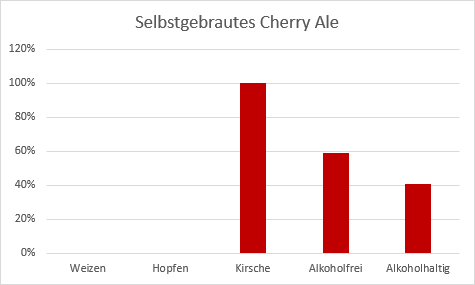
\includegraphics[width=0.5\columnwidth]{sca.png}
	\caption{Cherry Ale Tabelle}
\end{figure}
Das Cherry Ale wurde eindeutig als solches erkannt.
 Darüber hinaus wurde es auch von vielen als alkoholfreies Bier bezeichnet. Bei Rückfragen mit den Testpersonen ist uns klar geworden, dass das Cherry Ale im Allgemeinen nicht so beliebt ist. Dazu kam noch, dass viele der Testpersonen noch nie ein Cherry Ale probiert haben. Somit gab es auch ein grosses Misstrauen, dass dieses Bier wirklich alkoholhaltig ist.
 \begin{figure}[!h]
	\centering
	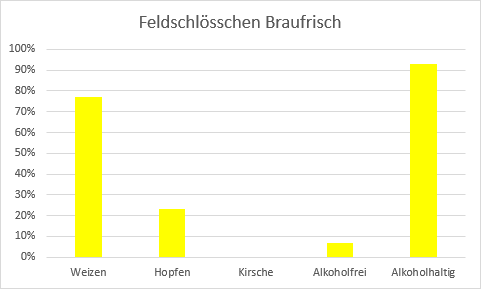
\includegraphics[width=0.5\columnwidth]{braufrish.png}
	\caption{Braufrisch Tabelle}
\end{figure}
Die Auswertung vom Feldschlösschen Braufrisch hat uns nicht sehr überrascht. Es ist ein sehr bekanntes und beliebtes Bier im Baselbiet. Somit viel die Bewertung natürlich auch sehr positiv aus. Eine klare Mehrheit der Befragten konnte erkennten, dass es sich um ein Weizenbier handelt. Der Unterschied, wieso so viele das Bier richtig erkennen konnten, ist, weil viele das Bier schon öfters konsumiert haben und ihnen der Geschmack somit gut bekannt ist. Auch bei der Frage ob da
s Bier alkoholhaltig ist, haben fast alle die richtige Antwort gegeben. 
\begin{figure}[!h]
	\centering
	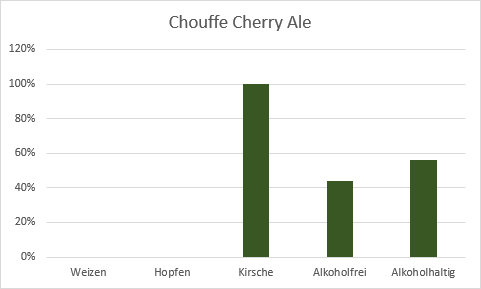
\includegraphics[width=0.5\columnwidth]{chouf.png}
	\caption{Chouffe Cherry Ale Tabelle}
\end{figure}
Nach der Auswertung unseres Cherry Ales war die Auswertung von dem Chouffe Cherry Ale nicht besonders überrascht. Auch hier war es eindeutig, dass es ein Kirschen Bier ist. Anders sieht es beim Alkoholgehalt aus. Hier erkannten mehr Befragte, dass es Alkoholhaltig ist. Hier wurde bei Rückfragen herausgefunden, dass man einen starken Unterschied zwischen unserem selbstgebrauten und dem gekauften Cherry Ale geschmeckt hat.
\begin{figure}[!h]
	\centering
	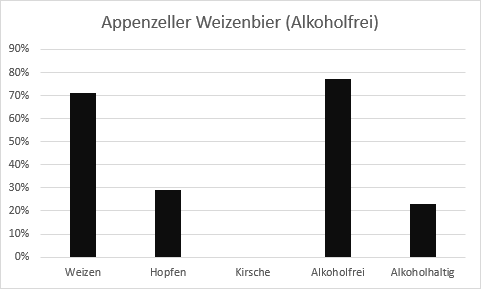
\includegraphics[width=0.5\columnwidth]{alkfree.png}
	\caption{Alkoholfreies Tabelle}
\end{figure}
Hier wussten 71 Prozent
dass es sich um ein Weizenbier handelt. 29 Prozent dachten es sei ein Hopfenbier. Hier könne der Grund dafür sein, dass es kein Alkohol in dem Bier hatte. Genau wissen wir es jedoch nicht. Wie man sehen kann wussten fast 80 Prozent der Befragten, dass es sich hierbei um ein alkoholfreies Bier handelt. Bei Rückfragen hat sich ergeben, dass man nach so vielen alkoholhaltigen Getränken sehr leicht das alkoholfreie Getränk erraten konnte. 
 
\begin{figure}[!h]
	\centering
	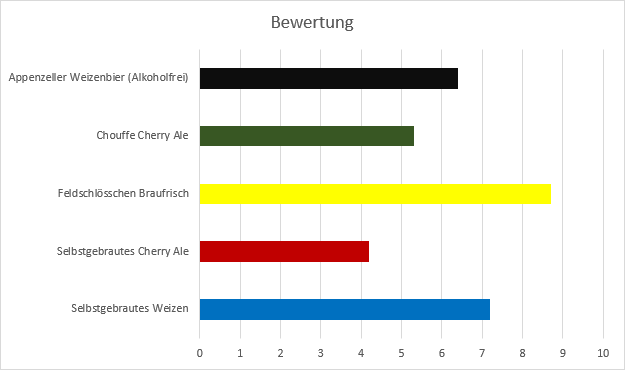
\includegraphics[width=0.5\columnwidth]{bewertung.png}
	\caption{Bewertung Tabelle}
\end{figure}
Wie man sehen kann ist das Feldschlösschen Bier das bestbewertetste Bier bei der Degustation. Das hat uns nicht überrasche. Weiter wurde unser Weizenbier aber als zweitbestes Bier bewertet. Wir sind stolz auf unsere Leistung. Wir selbst fanden sogar unser eigenes Bier besser als das von Feldschlösschen. Das Cherry Ale wurde allgemein schlechter bewertet, weil die Nachfrage dafür nicht sehr gross ist. Uns selbst hingegen hat das Cherry Ale noch sehr gut geschmeckt. 

\newpage
\subsection{Brauereibesuch}
\subsubsection{Ziele}
\begin{itemize}
  \item Wie wird das Bier in Gross- und Kleinbrauereien hergestellt?
  \item Welche Unterschiede gibt es zu dem Heimbrauen?
\end{itemize}



Wir haben uns dazu entschieden, ein Klein- und Grossbrauerei zu besuchen, um zu sehen, wie die Bierbrauerei dort aussieht. Dafür haben wir schon früh angefangen verschiedene Brauereien anzurufen. Bei vielen konnten wir mit dem Telefonat nur die E-Mail-Adresse der zuständigen Person herausfinden. Andere Brauereien, vor allem Kleinbrauereien haben uns aufgrund von COVID-19 sofort abgesagt. Das hat uns nichts ausgemacht, da wir auch einige Mailadressen bekommen haben. Wir konnten uns dann komplett auf diese Mails konzentrieren. Bevor wir die Mails formulierten, haben wir uns immer noch kurz über die Firma informiert, damit wir jeweils eine persönliche Anfrage formulieren konnten. Trotz unserer Bemühungen hat uns bereits noch am gleichen Tag eine Brauerei auch aufgrund von COVID-19 abgesagt. Nach drei weiteren Tagen hat uns eine weitere Brauerei abgesagt. Das war sogar eine Grossbrauerei, bei denen wir beim Anruf einen sehr guten Eindruck hatten. Danach hing unsere Hoffnung nur noch an einer Kleinbrauerei. Diese hat uns längere Zeit keine Antwort geschickt. Bei einem erneuten Anruf hat uns eine Sekretärin gesagt, dass die zuständige Person gerade sehr beschäftigt ist und dass wir evtl. eine Erinnerungs-Mail schreiben sollen. Auch auf diese Mail haben wir länger keine Antwort erhalten. Schlussendlich mussten wir auch diese Brauerei aufgeben. \\\\
Am 20.11.2020 kam auf dem Sender «SRF»  im Fernsehen die Sendung «Mini Schwiz dini Schwiz» dort hat eine Kandidatin den Ort «Laufen» im Baselland vorgestellt. Die Kandidatin hat Ihren Gästen im Verlauf der Sendung Ihr Hobby vorgestellt, das Bierbrauen. Leider war der Ausschnitt nur kurz aber wir haben uns den Ausschnitt dann gemeinsam im Nachhinein unter folgendem Link angesehen: \\\\
https://www.srf.ch/play/tv/mini-schwiiz-dini-schwiiz/video/basel-landschaft--tag-5---laufen?urn=urn:srf:video:cba25218-2d37-48a8-af7a-1489e28eb5c7
Minute: 16:53\\\\
In dem kurzen Ausschnitt hat er ganz rudimentär den Ablauf vom Bierbrauen erklärt. Dabei konnten wir verschiedene Behälter und Anlagen sehen. Auf diese sind Sie jedoch in der Sendung nicht weiter eingegangen. Zum Schluss konnten wir beobachten, wie sie das Bier in die Flaschen abgefüllt haben und die Labels aufgeklebt haben.
Nachdem wir den Ausschnitt gesehen haben, wollten wir es noch bei dieser Brauerei versuchen und haben vom Kontaktformular der Homepage www.birsfallbier.ch eine Mail geschrieben. Auf diese Mail haben wir bislang keine Antwort bekommen. Wir sind aber zuversichtlich und hoffen, dass wir bis zum Präsentationstermin der VA noch eine Antwort erhalten. Wir haben uns in der Mail nicht direkt auf einen Besuch bezogen, da dies bei den anderen Brauereien nie gut ankam. Wir wollten lediglich ein Interview, in dem wir Fragen über das Bierbrauen in grösseren Mengen stellen könnten.

\newpage